%% LyX 2.2.2 created this file.  For more info, see http://www.lyx.org/.
%% Do not edit unless you really know what you are doing.
\documentclass[english]{article}
\usepackage{lmodern}
\usepackage[T1]{fontenc}
\usepackage[utf8]{inputenc}
\usepackage{color}
\usepackage{babel}
\usepackage{amsmath}
\usepackage{amsthm}
\usepackage{amssymb}
\usepackage{graphicx}
\usepackage[numbers]{natbib}
\usepackage[unicode=true,pdfusetitle,
 bookmarks=true,bookmarksnumbered=false,bookmarksopen=false,
 breaklinks=false,pdfborder={0 0 1},backref=false,colorlinks=false]
 {hyperref}
\usepackage{breakurl}

\makeatletter
%%%%%%%%%%%%%%%%%%%%%%%%%%%%%% User specified LaTeX commands.
%\usepackage[utf8]{inputenc}
\usepackage{verbatim}

\makeatother

\begin{document}


\section{Q-learning}

In Reinforcement Learning we are interested in maximizing the \emph{Expected
Return} so we usually work directly with those expectations. For instance,
in \emph{Q-learning }with \emph{function approximation} we want to
minimize the error
\[
\mathbb{E}_{s,a}\left[\left(r(s,a)+\gamma\mathbb{E}_{s'}\left[\max_{a'}Q(s',a')\right]-Q(s,a)\right)^{2}\right],
\]
or, equivalently,
$$\begin{align}
\mathbb{E}_{s,a,s'}\left[\left(r(s,a)+\gamma\max_{a'}Q(s',a')-Q(s,a)\right)^{2}\right],\label{eq:classic_td_error}
\end{align}$$
where $r(s,a)$ is the \emph{expected immediate reward}. In \emph{semi-gradient
}methods we do this by moving $Q(s,a)$ towards the \emph{target}
$r(s,a)+\gamma\max_{a'}Q(s',a')$, pretending that the target is constant,
and in \emph{DQN\citep{mnih2015human}} we even \emph{freeze }the
``target network'' to improve stability even further.

The main idea of \emph{Distributional RL\citep{DBLP:journals/corr/BellemareDM17}
}is to work directly with the \emph{full distribution} of the return
rather than with its expectation. Let the random variable $Z(s,a)$
be the return obtained by starting from state $s$, performing action
$a$ and then following the current policy. Then
\[
Q(s,a)=\mathbb{E}[Z(s,a)].
\]
Instead of trying to minimize the error~$\ref{eq:classic_td_error}$,
which is basically a distance between expectations, we can instead
try to minimize a \emph{distributional }error, which is a distance
between full distributions:
$$\begin{align}
\sup_{s,a}\mathrm{dist}\left(R(s,a)+\gamma Z(s',a^{*}),Z(s,a)\right)\label{eq:distrib_td_error}\\
s'\sim p(\cdot|s,a)\nonumber 
\end{align}$$
where you can mentally replace $\sup$ with $\max$, $R(s,a)$ is
the random variable for the immediate reward, and
\[
a^{*}=\underset{a'}{\mathrm{arg\,max}\,}Q(s',a')=\underset{a'}{\mathrm{arg\,max}\,}\mathbb{E}[Z(s',a')].
\]
Note that we're still using $Q(s,a)$, i.e. the expected return, to
decide which action to pick, but we're trying to optimize \emph{distributions}
rather than \emph{expectations} (of those distributions).

There's a subtlety in expression~$\ref{eq:distrib_td_error}$: if $s,a$
are constant, $Z(s,a)$ is a random variable, but even more so when
$s$ or $a$ are themselves random variables!

\section{Policy Evaluation}

Let's consider \emph{policy evaluation} for a moment. In this case
we want to minimize
\[
\mathbb{E}_{s,a,s',a'}\left[\left(r(s,a)+\gamma Q(s',a')-Q(s,a)\right)^{2}\right]
\]
We can define the \emph{Bellman operator} \emph{for evaluation} as
follows:
\[
(\mathcal{T}^{\pi}Q)(s,a)=\mathbb{E}_{s'\sim p(\cdot|s,a),a'\sim\pi(\cdot|s')}[r(s,a)+\gamma Q(s',a')]
\]
The Bellman operator $\mathcal{T}^{\pi}$ is a $\gamma$\emph{-contraction},
meaning that
\[
\mathrm{dist}\left(\mathcal{T}Q_{1},\mathcal{T}Q_{2}\right)\leq\gamma\mathrm{dist}\left(Q_{1},Q_{2}\right),
\]
so, since $Q^{\pi}$ is a \emph{unique }fixed point (i.e. $\mathcal{T}Q=Q\iff Q=Q^{\pi}$),
we must have that $\mathcal{T}^{\infty}Q=Q^{\pi}$, disregarding approximation
errors.

It turns out \citep{DBLP:journals/corr/BellemareDM17} that this result
can be ported to the distributional setting. Let's define the \emph{Bellman
distribution operator for evaluation} in an analogous way:
$$\begin{align*}
(\mathcal{T}_{D}^{\pi}Z)(s,a) & =R(s,a)+\gamma Z(s',a')\\
s' & \sim p(\cdot|s,a)\\
a' & \sim\pi(\cdot|s')
\end{align*}$$
$\mathcal{T}_{D}^{\pi}$ is a \emph{$\gamma$-contraction} in the
\emph{Wasserstein distance $\mathcal{W}$, i.e.
\[
\sup_{s,a}\mathcal{W}\left(\mathcal{T}_{D}^{\pi}Z_{1}(s,a),\mathcal{T}_{D}^{\pi}Z_{2}(s,a)\right)\leq\gamma\sup_{s,a}\mathcal{W}(Z_{1}(s,a),Z_{2}(s,a))
\]
}This isn't true for the \emph{KL divergence}.

Unfortunately, this result doesn't hold for the \emph{control} (the
one with the $\max$) version of the distributional operator.

\section{KL divergence}

\subsection{Definition}

I warn you that this subsection is \emph{highly informal.}

If $p$ and $q$ are two distributions with same \emph{support} (i.e.
their \emph{pdfs} are non-zero at the same points), then their KL
divergence is defined as follows:
\[
\mathrm{KL}(p\|q)=\int p(x)\log\frac{p(x)}{q(x)}dx.
\]

Let's consider the \emph{discrete} case:
\[
\mathrm{KL}(p\|q)=\sum_{i=1}^{N}p(x_{i})\log\frac{p(x_{i})}{q(x_{i})}=\sum_{i=1}^{N}p(x_{i})[\log p(x_{i})-\log q(x_{i})].
\]
As we can see, we're basically comparing the \emph{scores} at the
points $x_{1},\ldots,x_{N}$, weighting each comparison according
to $p(x_{i})$. Note that the KL doesn't make use of the values $x_{i}$
directly: only their probabilities are used! Moreover, if $p$ and
$q$ have different supports, the KL is undefined.

\subsection{How to use it}

Now say we're using DQN and extract $(s,a,r,s')$ from the \emph{replay
buffer}. A \emph{sample }of the target distribution is $r+\gamma Z(s',a^{*})$,
where $a^{*}=\mathrm{arg\,max}_{a'}Q(s',a')$. We want to move $Z(s,a)$
towards this target (by keeping the target fixed).

I called $r+\gamma Z(s',a^{*})$ a \emph{sample} of a distribution,
which might sound like a contradiction in terms, but it isn't. This
is just a sample because $r$ and $s'$ are not random variables,
but just samples. We still get a distribution though since $Z(s',a^{*})$
is a distribution. Indeed, to get a \emph{single} sample \textbf{\emph{from}}
the \emph{real} distribution, we should first sample $r$ and $s'$,
and, finally, sample from the distribution $r+\gamma Z(s',a^{*})$.
Note that this is almost exactly what we're doing since $r$ and $s'$
extracted from the replay buffer were indeed sampled. The only difference
is that instead of sampling from $r+\gamma Z(s',a^{*})$, we use the
full distribution (but based, again, on just samples of $r$ and $s'$).

Let's say we have a net which models $Z$ by taking a state $s$ and
returning a distribution $Z(s,a)$ for each action. For instance,
we can represent each distribution through a \emph{softmax} like we
often do in \emph{Deep Learning} for \emph{classification tasks}.
In particular, let's choose some fixed values $x_{1},\ldots,x_{N}$
for the support of all the distributions returned by the net. To simplify
things, let's make them \emph{equidistant} so that
\[
x_{i+1}-x_{i}=d=(x_{N}-x_{1})/(N-1),\qquad i=1,\ldots,N-1
\]
The pmf looks like a comb:
\begin{center}
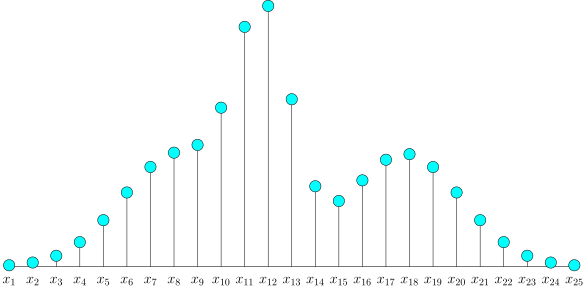
\includegraphics[width=1\textwidth]{discrete}
\par\end{center}

Since the values $x_{1},\ldots,x_{N}$ are fixed, we just have to
return $N$ probabilities for each $Z(s,a)$, so the net takes a single
state and returns $|\mathcal{A}|N$ scalars, where $|\mathcal{A}|$
is the number of possible actions.

If $p_{1},\ldots,p_{N}$ and $q_{1},\ldots,q_{N}$ are the probabilities
of the two distributions $p$ and $q$, then their KL is simply
\[
\mathrm{KL}(p\|q)=\sum_{i=1}^{N}p_{i}\log\frac{p_{i}}{q_{i}}=H(p,q)-H(p)
\]
and if you're optimizing wrt $q$ (i.e. you're moving $q$ towards
$p$), then you can drop the \emph{entropy }term.

Also, we can recover $Q(s,a)$ very easily:
\[
Q(s,a)=\mathbb{E}[Z(s,a)]=\sum_{i=1}^{N}p_{i}x_{i}.
\]

The interesting part is the \emph{transformation}. In distributional
Q-learning we want to move $Z(s,a)$ towards $r+\gamma Z(s',a^{*})$,
but how do we put $p$ in ``standard comb form''? This is the \emph{projection
part} described in \citep{DBLP:journals/corr/BellemareDM17} and it's
very easy. To form the target distribution we start from $p=Z(s',a^{*})$,
which is already in the standard form $p_{1},\ldots,p_{N}$ and we
look at the pairs $(x_{1},p_{1}),\ldots,(x_{N},p_{N})$ as if they
represented \emph{samples }with \emph{weights}, which the authors
of \citep{DBLP:journals/corr/BellemareDM17} call \emph{atoms}. This
means that we can transform the distribution $p$ just by transforming
the position of its \emph{atoms}. The transformed atoms corresponding
to $r+\gamma Z(s',a^{*})$ are
\[
(r+\gamma x_{1},p_{1}),(r+\gamma x_{2},p_{2}),\ldots,(r+\gamma x_{N},p_{N}).
\]
Note that the weights $p_{i}$ don't change. The problem is that now
we have atoms which aren't in the standard positions $x_{1},\ldots,x_{N}$.
The solution proposed in~\citep{DBLP:journals/corr/BellemareDM17}
is to \emph{split} each \emph{misaligned} atom into the two closest
\emph{aligned} atoms by making sure to distribute its weight according
to its distance from the two misaligned atoms:
\begin{center}
\begin{figure}
\begin{centering}
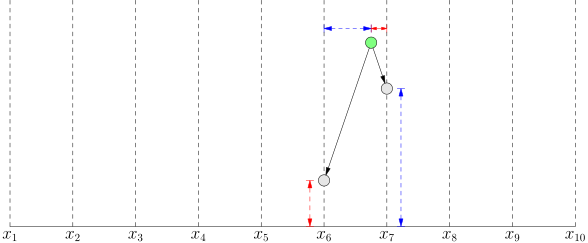
\includegraphics[width=1\textwidth]{split}
\par\end{centering}
\caption{\label{fig:atom_splitting}}
\end{figure}
\par\end{center}

Observe the proportions very carefully. Let's say the \textcolor{green}{green}
atom has weight $w.$ For some constants $c$, the \textcolor{green}{green}
atom is at distance $3c$ from $x_{6}$ and $c$ from $x_{7}$. Indeed,
the atom at $x_{6}$ receives weight $\frac{1}{4}w$ and the atom
at $x_{7}$ weight $\frac{3}{4}w$, which makes sense. Also, note
that the \emph{probability mass} is conserved so there's no need to
normalize after the splitting. Of course, since we need to split all
the transformed atoms, individual aligned atoms can receive contributions
from different atoms. We simply sum all the contributions. This is
how the authors do it, but it's certainly not the only way.

\subsection{The full algorithm}

Here's the algorithm taken directly (cut \& pasted) from \citep{DBLP:journals/corr/BellemareDM17}:
\begin{center}
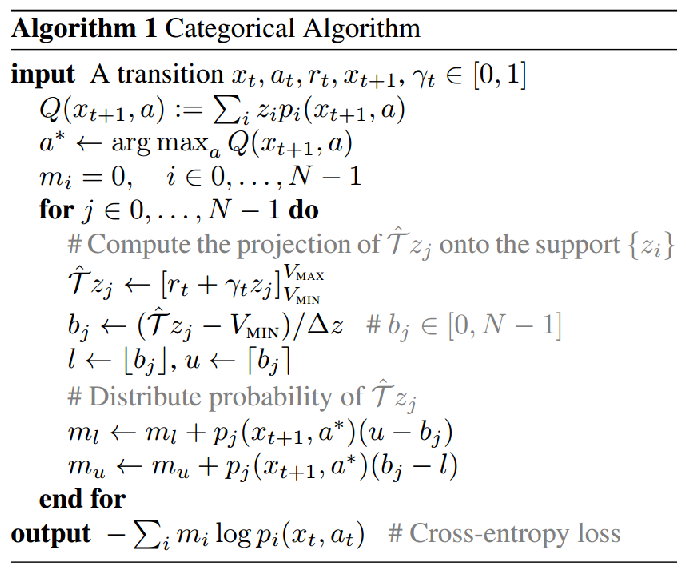
\includegraphics[width=0.7\textwidth]{KL_algo}
\par\end{center}

Assume we've just picked $(x_{t},a_{t},r_{t},x_{t+1})$ from the \emph{replay
buffer} in some variant of the DQN algorithm, so $x$ is used to indicate
\emph{states}. The $z_{0},\ldots,z_{N-1}$ are the fixed global positions
of the atoms (i.e. our $x_{1},\ldots,x_{N}$ in figure~$\ref{fig:atom_splitting}$).
Let's assume there's just a global $\gamma$.

Let's go through the algorithm in detail assuming we're using a neural
network for $Z$:
\begin{enumerate}
\item We fead $x_{t+1}$ to our net which outputs an $|\mathcal{A}|\times N$
matrix $M(x_{t+1})$, i.e. each row corresponds to a single action
and contains the probabilities for the $N$ atoms. That is, the row
for action $a$ contains the vector
\[
(p_{0}(x_{t+1},a),\ldots,p_{N-1}(x_{t+1},a))
\]
\item We compute all the 
\[
Q(x_{t+1},a)=\mathbb{E}\left[Z(x_{t+1},a)\right]=\sum_{i=0}^{N-1}z_{i}p_{i}(x_{t+1},a)
\]
as follows:
\[
Q(x_{t+1})=M(x_{t+1})\begin{bmatrix}z_{0}\\
z_{1}\\
\vdots\\
z_{N-1}
\end{bmatrix}.
\]
Note that $Q(x_{t+1})$ is a column vector of length $|\mathcal{A}|$.
\item Now we can determine the optimum action
\[
a^{*}=\mathrm{arg\,max_{a}}Q(x_{t+1},a)
\]
Let $q=(q_{0},\ldots,q_{N-1})$ be the row of $M(x_{t+1})$ corresponding
to $a^{*}$.
\item $m_{0},\ldots,m_{N-1}$ will accumulate the probabilities of the \emph{aligned}
atoms of the target distribution $r_{t}+\gamma Z(x_{t+1},a^{*})$.
We start by zeroing them.
\item The \emph{non-aligned} atoms of the target distribution are at positions
\[
\hat{\mathcal{T}}z_{j}=r_{t}+\gamma z_{j},\qquad j=0,\ldots,N-1
\]
 We clip those positions so that they are in $[V_{\mathrm{MIN}},V_{\mathrm{MAX}}]$,
i.e. $[z_{0},z_{N-1}]$.
\item Assuming that the adjacent aligned atoms are at distance $\Delta z$,
the indices of the closest \emph{aligned} atoms on the left and on
the right of $\hat{\mathcal{T}}z_{j}$ are, respectively:
$$\begin{align*}
l & =\left\lfloor \frac{\hat{\mathcal{T}}z_{j}-z_{0}}{\Delta z}\right\rfloor \\
u & =\left\lceil \frac{\hat{\mathcal{T}}z_{j}-z_{0}}{\Delta z}\right\rceil 
\end{align*}$$
\item Now we need to split the weight of $\hat{\mathcal{T}}z_{j}$, which
is $q_{j}$, between $m_{l}$ and $m_{r}$ as we saw before. Note
that
$$\begin{align*}
(u)-(b_{j}) & =\left(\frac{z_{u}-z_{0}}{\Delta z}\right)-\left(\frac{\hat{\mathcal{T}}z_{j}-z_{0}}{\Delta z}\right)=\frac{z_{u}-\hat{\mathcal{T}}z_{j}}{z_{u}-z_{l}}\\
(b_{j})-(l) & =\left(\frac{\hat{\mathcal{T}}z_{j}-z_{0}}{\Delta z}\right)-\left(\frac{z_{l}-z_{0}}{\Delta z}\right)=\frac{\hat{\mathcal{T}}z_{j}-z_{l}}{z_{u}-z_{l}}
\end{align*}$$
which means that, as we said before, the weight $q_{j}$ is split
between $z_{l}$ and $z_{u}$ (indeed, $u-b_{j}+b_{j}-l=1)$, and
the contribution to $m_{l}$ is proportional to the distance of $\hat{\mathcal{T}}z_{j}$
from $z_{u}$. The more distant it is from $z_{u}$, the higher the
contribution to $m_{l}$.
\item Now we have the probabilities $m_{0},\ldots,m_{N-1}$ of the \emph{aligned}
atoms of $r_{t}+\gamma Z(x_{t+1},a^{*})$ and, of course, the probabilities
\[
p_{0}(x_{t},a_{t};\theta),\ldots,p_{N-1}(x_{t},a_{t};\theta)
\]
of the \emph{aligned} atoms of $Z(x_{t},a)$, which are the ones we
want to update. Thus
$$\begin{align*}
\nabla_{\theta}\mathrm{KL}(m\|p_{\theta}) & =\nabla_{\theta}\sum_{i=0}^{N-1}m_{i}\log\frac{m_{i}}{p_{\theta}}\\
 & =\nabla_{\theta}\left[H(m,p_{\theta})-H(m)\right]\\
 & =\nabla_{\theta}H(m,p_{\theta})
\end{align*}$$
That is, we can just use the \emph{cross-entropy}
\[
H(m,p_{\theta})=-\sum_{i=0}^{N-1}m_{i}\log p_{i}(x_{t},a_{t};\theta)
\]
for the \emph{loss}.
\end{enumerate}
%

\section{Wasserstein distance}

The first paper \citep{DBLP:journals/corr/BellemareDM17} about \emph{distributional
RL} left a \emph{gap} between theory and practice because the theory
requires the \emph{Wasserstein distance}, but in practice they used
a KL-based procedure.

The second paper \citep{2017arXiv171010044D} closes the gap in a
very elegant way.

\subsection{A different idea\label{subsec:A-different-idea}}

This time I won't start with a definition, but with an \emph{idea}.
Rather than use atoms with \emph{fixed positions}, but \emph{variable
weights}, let's do the opposite: let's use atoms with \emph{fixed
weights}, but \emph{variable positions}. Moreover, let's use the same
weight for each atom, i.e. $1/N$ if the atoms are $N$.

But how do we represent distributions this way? It's very simple,
really. We slice up the distribution we want to represent into $N$
slices of $1/N$ mass and put each atom at the \emph{median} of a
slice. This makes sense; in fact, the atoms weigh $1/N$ as well:

\begin{figure}
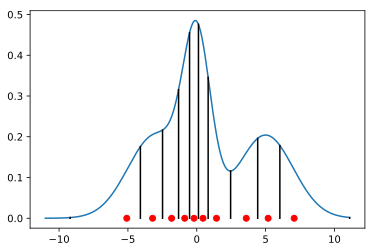
\includegraphics[width=0.9\textwidth]{quantiles}

\caption{The distribution has been sliced up into slices of equal \emph{probability
mass} and red points have been placed in the center of mass of each
slice. For the code, see subsection~$\ref{subsec:Some-code}$. This
image is produced through sampling as described in the following sections.\label{fig:sliced_up_distrib}}
\end{figure}

If the atoms are $N$ then the $i$-th atom corresponds to a quantile
of
\[
\hat{\tau}_{i}=\frac{2(i-1)+1}{2N},\qquad i=1,\ldots,N
\]


\subsection{How do we determine a quantile?}

\subsubsection{Determining the median}

The median is just the \emph{$0.5$ quantile}, i.e. a point which
has $0.5$ mass on the left and $0.5$ mass on the right. In other
words, it splits the probability mass in half. So let's say we have
a random variable $X$ and we know how to draw samples. How can we
compute the median? We start with a guess $\theta$, draw some samples
and if $\theta$ has more samples on the left than on the right, we
move it a little to the left. By symmetry, we move it to the right
if it has more samples on the right. Then we repeat the process and
keep updating $\theta$ until convergence.

We should move $\theta$ in proportion to the disparity between the
two sides, so let's decide that each sample on the \emph{left} subtract
$\alpha$ and each sample on the \emph{right} add $\alpha$. Basically,
$\alpha$ is a \emph{learning rate}. If it's too small the algorithm
takes too long and if it's too big the algorithm \emph{fluctuates
}a lot around the optimal solution. Here's a picture about this method:
\begin{center}
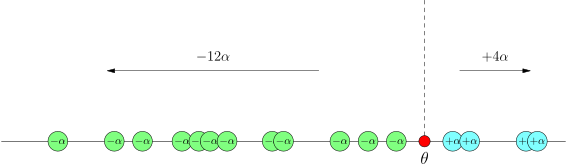
\includegraphics[width=1\textwidth]{median}
\par\end{center}

We reach the equilibrium when $\theta$ is the median. Doesn't this
look like \emph{SGD} with a \emph{minibatch} of $16$ samples and
learning rate $\alpha$? What's the corresponding \emph{loss}? The
loss is clearly
\begin{equation}
L_{\theta}=\mathbb{E}_{X}[|X-\theta|]\label{eq:median_loss}
\end{equation}
This should look familiar to any statistician. Note that in the picture
above we're adding the gradients, but when we \emph{minimize} we subtract
them so gradients on the left of $\theta$ must be $1$ and on the
right $-1$:
\[
\nabla_{\theta}L_{\theta}=\begin{cases}
\nabla_{\theta}(\theta-X)=1 & \text{if }X<\theta\\
\nabla_{\theta}(X-\theta)=-1 & \text{if }X\geq\theta
\end{cases}
\]


\subsubsection{Determining any quantile}

We can generalize this to any quantile by using different \emph{weights}
for the left and right samples. Let's omit the $\alpha$ for more
clarity, since we know it's just the learning rate by now. If we want
the probability mass on the left of $\theta$ to be $\tau$, we need
to use weight $1-\tau$ for the samples on the left and $\tau$ for
the ones on the right. This works because, when $\theta$ is the $\tau$
quantile, if we sample $S$ samples then, \emph{on average}, the samples
on the left will be $\tau S$ and the ones on the right $(1-\tau)S$.
Multiplying the number of samples by their weights, we get an equality:
\[
(\tau S)(1-\tau)=((1-\tau)S)(\tau)
\]
so both sides \emph{pull }with equal strength \emph{if and only if
}$\theta$ is the $\tau$ quantile.

Basically, we need to scale the weights/gradients on the left of $\theta$
by $1-\tau$ and the ones on the right by $\tau$, which are both
nonnegative scalars, since $\tau\in[0,1]$. Here's a compact expression
for that:
\[
|\tau-\delta_{X<\theta}|=\begin{cases}
|\tau-1|=1-\tau & \text{if }X<\theta\\
\tau & \text{if }X\geq\theta
\end{cases}
\]
Therefore, we just need to multiply the $|X-\theta|$ in the loss~$\ref{eq:median_loss}$
by $|\tau-\delta_{X<\theta}|$:
$$\begin{align*}
L_{\theta} & =\mathbb{E}_{X}[|X-\theta||\tau-\delta_{X<\theta}|]\\
 & =\mathbb{E}_{X}[\rho_{\tau}(X-\theta)]
\end{align*}$$
where
$$\begin{align}
\rho_{\tau}(u) & =|u||\tau-\delta_{u<0}|\label{eq:rho_t_abs}\\
 & =u(\tau-\delta_{u<0})\label{eq:rho_t_no_abs}
\end{align}$$
Note that we can eliminate the two absolute values because the two
factors have always the same sign. Expression~$\ref{eq:rho_t_no_abs}$
is the one we find in equation (8) in \citep{2017arXiv171010044D},
but expression~$\ref{eq:rho_t_abs}$ makes it clearer that we can eliminate
the \emph{cuspid} in $\rho_{t}$ by replacing $|u|$ with the \emph{Huber
loss} defined as:
\[
\mathcal{L}_{\kappa}(u)=\begin{cases}
\frac{1}{2}u^{2} & \text{if }|u|\leq\kappa\\
\kappa(|u|-\frac{1}{2}\kappa) & \text{otherwise }
\end{cases}
\]
This makes optimization easier, according to the authors of \citep{2017arXiv171010044D}.
We're interested in $\mathcal{L}_{1}$ in particular because it's
the only one with the right slopes in the \emph{linear parts}. Here's
a picture of the two curves:

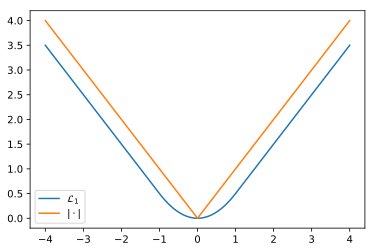
\includegraphics[width=0.8\textwidth]{rho_05}

Now we can define $\rho_{\kappa}$ as follows:
$$\begin{align*}
\rho_{\tau}^{0}(u) & =\rho_{\tau}(u)=u(\tau-\delta_{u<0})\\
\rho_{\tau}^{\kappa}(u) & =\mathcal{L}_{\kappa}(u)|\tau-\delta_{u<0}|
\end{align*}$$

Here's a picture of $\rho_{0.3}$ and $\rho_{0.3}^{1}$:

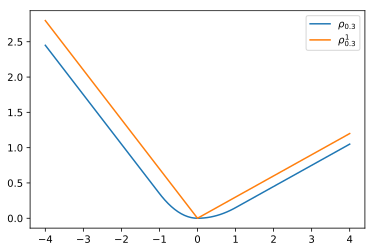
\includegraphics[width=0.8\textwidth]{rho_03}

The final loss becomes
\[
L_{\theta}=\mathbb{E}_{X}[\rho_{\tau}^{1}(X-\theta)]
\]


\subsubsection{Computing all the needed quantiles at once}

To compute more quantiles at once, we can just compute the total loss
given by
\[
L_{\theta}=\sum_{i=1}^{N}\mathbb{E}_{X}[\rho_{\tau_{i}}^{1}(X-\theta_{i})]
\]
where $\theta=(\theta_{1},\ldots,\theta_{N})$ and we want $\theta_{i}$
to be the $\tau_{i}$ quantile. Of course, in general we can write
\begin{equation}
L_{\theta}=\sum_{i=1}^{N}\mathbb{E}_{X}[\rho_{\tau_{i}}^{1}(X-f(\theta)_{i}]\label{eq:q_reg_formula}
\end{equation}
where $f$ is some $\mathbb{R}^{N}$-valued function of $\theta$.

\subsubsection{Some code\label{subsec:Some-code}}

Here's the code for drawing picture~$\ref{fig:sliced_up_distrib}$
in subsection~$\ref{subsec:A-different-idea}$:

\begin{verbatim}
%%%%lyxblog-raw

import tensorflow as tf
import matplotlib.pyplot as plt
import numpy as np


class Quantiles:
    def __init__(self, taus, tf_graph=None):
        self.taus = taus
        N = len(taus)

        graph = tf_graph or tf.get_default_graph()
        with graph.as_default():
            with tf.variable_scope('quantiles'):
                self.xs = tf.placeholder('float')
                self.theta = tf.get_variable('theta', shape=(N,))
                self.loss = sum(
                    tf.reduce_mean(self._rho_tau(self.xs - self.theta[i],
                                                 taus[i], kappa=0))
                    for i in range(N))
                self.train_step = tf.train.AdamOptimizer(0.05).minimize(
                    self.loss)

    @staticmethod
    def _HL(u, kappa):
        delta = tf.cast(abs(u) <= kappa, 'float')
        return delta * (u * u / 2) + (1 - delta) * (
                kappa * (abs(u) - kappa / 2))

    @staticmethod
    def _rho_tau(u, tau, kappa=1):
        delta = tf.cast(u < 0, 'float')
        if kappa == 0:
            return (tau - delta) * u
        else:
            return abs(tau - delta) * Quantiles._HL(u, kappa)

    def get_quantiles(self, samples, loops):
        with tf.Session() as sess:
            tf.global_variables_initializer().run()
            for _ in range(loops):
                loss, _ = sess.run([self.loss, self.train_step],
                                   {self.xs: samples})
            qs = sess.run(self.theta)
        return qs


class MixtureOfGaussians:
    def __init__(self, pis, mus, sigmas):
        self.pis = pis
        self.mus = mus
        self.sigmas = sigmas

    def draw_samples(self, n):
        samples = np.empty(n)
        for i in range(n):
            idx = np.random.multinomial(1, self.pis).argmax()
            samples[i] = np.random.normal(self.mus[idx], self.sigmas[idx])
        return samples

    def pdf(self, x):
        return np.sum(pi * np.exp(-0.5 * ((x - mu) / s) ** 2) /
                        (s * np.sqrt(2 * pi))
                      for pi, mu, s in zip(self.pis, self.mus, self.sigmas))


tf.reset_default_graph()

MoG = MixtureOfGaussians(pis=[1/3, 1/3, 1/3], mus=[-3, 0, 5], sigmas=[2, 1, 2])
xs = np.linspace(-11, 11, num=200)
ys = MoG.pdf(xs)

N = 10  # num of quantiles
taus = [i / (2 * N) for i in range(0, 2 * N + 1)]
Q = Quantiles(taus)
samples = MoG.draw_samples(10000)
qs = Q.get_quantiles(samples, loops=2000)

plt.plot(xs, ys)

for q in qs[::2]:
    plt.plot([q, q], [0, MoG.pdf(q)], 'black')
plt.plot(qs[1::2], np.zeros_like(qs[1::2]), 'or')

plt.savefig('quantiles.svg', bbox_inches='tight')
plt.show()

\end{verbatim}

\subsection{Definition of the Wasserstein metric}

Let $X$ and $Y$ be two \emph{scalar} random variables and $F_{X}$
and $F_{Y}$ their \emph{CDFs}. Then, their \emph{$p$-Wasserstein
distance} is
\[
\mathcal{W}_{p}(X,Y)=\left(\int_{0}^{1}\left|F_{X}^{-1}(u)-F_{Y}^{-1}(u)\right|^{p}du\right)^{1/p}
\]
We'll use the $1$-Wasserstein distance (i.e. with $p=1$) which measures
the difference between the CDFs by measuring the area of a ``discrepancy
region'' (the \textcolor{cyan}{cyan} region in the picture):

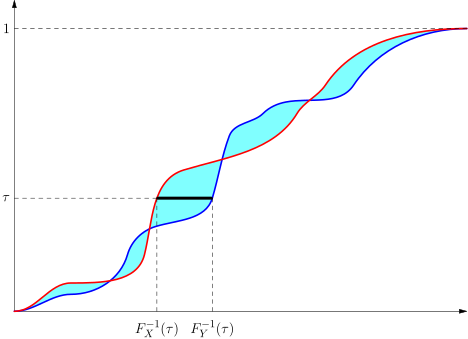
\includegraphics[width=0.8\textwidth]{wasserstein}

Now note that the CDF of a distribution represented by atoms $y_{1},\ldots,y_{N}$
of probability mass $q$ is a step function:

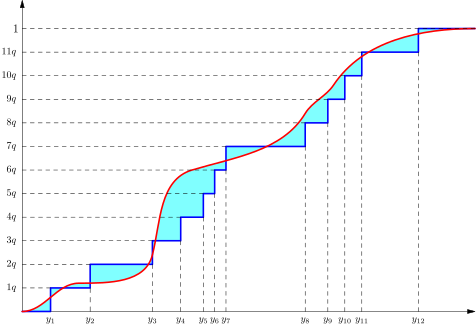
\includegraphics[width=0.8\textwidth]{wasserstein_step}

The \textcolor{cyan}{cyan }region, and thus the Wasserstein distance,
is reduced when we slice up the \textcolor{red}{red} curve into $q$-mass
slices and choose our atoms so that they halves the mass of each slice:

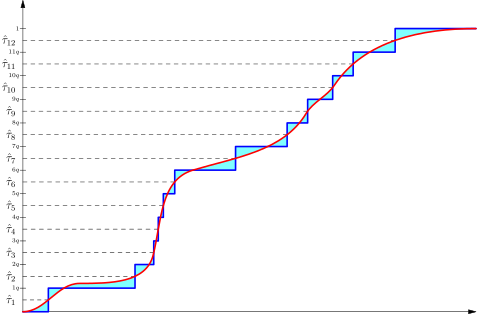
\includegraphics[width=0.8\textwidth]{wasserstein_optim}

Note that in the picture above
\[
\hat{\tau}_{i}=\frac{2(i-1)+1}{2N},\qquad i=1,\ldots,N
\]
with $N=12$. The positions of our atoms are
\[
y_{i}=F_{X}^{-1}(\hat{\tau}_{i}),\qquad i=1,\ldots,N
\]
where $X$ is the variable associated with the \textcolor{red}{red}
CDF.

Here's what we get with $30$ atoms:

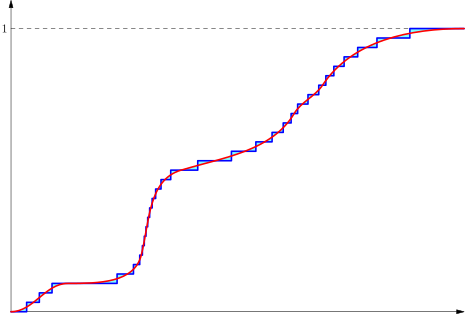
\includegraphics[width=0.8\textwidth]{wasserstein_optim_30}

So, it seems to be working!

\subsection{The full algorithm\label{subsec:The-full-algorithm}}

Here's the full algorithm taken directly (cut \& pasted) from \citep{2017arXiv171010044D}:

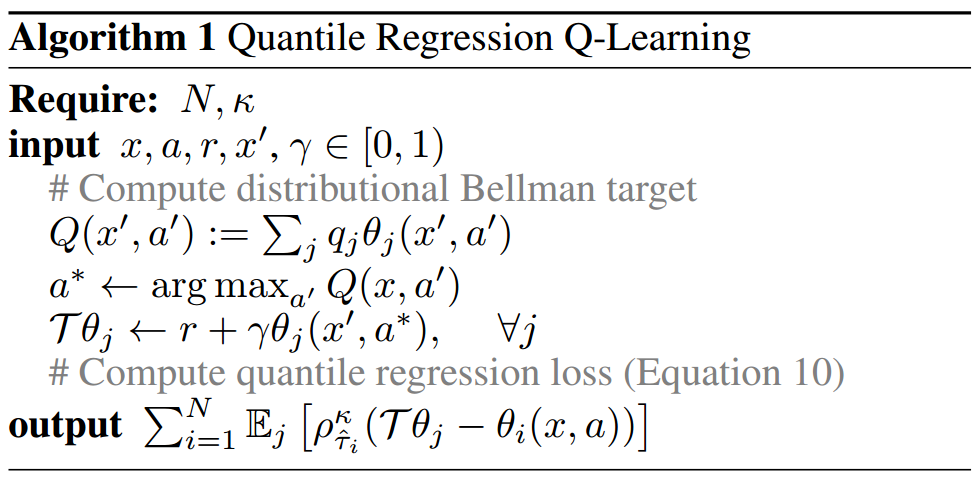
\includegraphics[width=0.7\textwidth]{W_algo}

As before, let's assume we've just picked $(x,a,r,x')$ from the \emph{replay
buffer} in some variant of the DQN algorithm, so $x$ is used to indicate
\emph{states}. The algorithm is quite simple:
\begin{enumerate}
\item We recover $Q(x')$ from $Z(x')$ returned by our net. We can assume
that $q_{j}=\frac{1}{N}$, i.e. the atoms have the same weight.
\item We find $a^{*}$ which is the optimal action according to $Q(x'$)
(there's a typo in the code).
\item Remember that the network, given a state ($x'$ in this case), returns
a \emph{matrix} where each row contains the $N$ atoms for a particular
action. Let $\theta'_{1},\ldots,\theta'_{N}$ be the atoms of $Z(x',a^{*})$.
\item We treat the atoms $\theta'_{1},\ldots,\theta'_{N}$ as samples and
transform them directly:
\[
\mathcal{T}\theta'_{j}=r+\gamma\theta'_{j},\qquad i=1,\ldots,N
\]
\item Let $\theta_{1},\ldots,\theta_{N}$ be the atoms of $Z(x,a)$. We
want to reduce the Wasserstein distance between $Z(x,a)$ and $r+\gamma Z(x',a^{*})$
by optimizing $Z(x,a)$. As always, the target $r+\gamma Z(x',a^{*})$
is treated as a constant for stability reasons (and we even use \emph{target
freezing} for extra stability).\\
We have $N$ samples for the target distribution, that is $\mathcal{T}\theta'_{1},\ldots,\mathcal{T}\theta'_{j}$.
So, we can use formula~$\ref{eq:q_reg_formula}$:
\[
L_{\theta}=\sum_{i=1}^{N}\mathbb{E}_{X}\left[\rho_{\tau_{i}}^{1}(X-f(\theta)_{i})\right]
\]
In our case, the formula becomes
$$\begin{align*}
L_{\theta} & =\sum_{i=1}^{N}\mathbb{E}_{X}\left[\rho_{\tau_{i}}^{1}(X-f(\theta)_{i})\right]\\
 & =\sum_{i=1}^{N}\mathbb{E}_{\mathcal{T}Z'}\left[\rho_{\hat{\tau}_{i}}^{1}(\mathcal{T}Z'-\theta_{i})\right],\qquad\mathcal{T}Z'=r+\gamma Z(x',a^{*})\\
 & =\frac{1}{N}\sum_{i=1}^{N}\sum_{j=1}^{N}\left[\rho_{\hat{\tau}_{i}}^{1}(\mathcal{T}\theta'_{j}-\theta_{i})\right]
\end{align*}$$
where
\[
\hat{\tau}_{i}=\frac{2(i-1)+1}{2N},\qquad i=1,\ldots,N
\]
\end{enumerate}

\subsection{Why don't we use simple regression?}

Both the \emph{``moving'' distribution} and the \emph{target distribution}
are represented by $N$ atoms each of weight $1/N$:

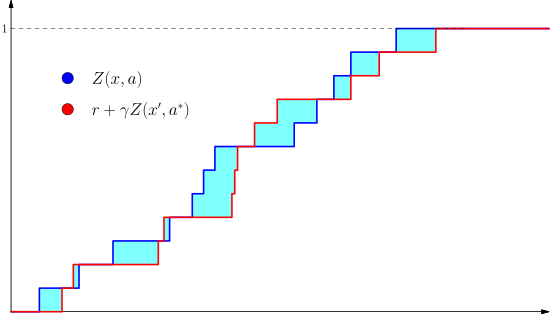
\includegraphics[width=0.8\textwidth]{wasserstein_both}

So why don't we avoid sampling and use simple regression? That is:
\begin{equation}
L_{\theta}=\sum_{i=1}^{N}(\theta_{i}-\theta'_{i})^{2}\label{eq:simple_reg_loss}
\end{equation}
The problem is that the atom positions $\theta_{1},\ldots,\theta_{N}$
and $\theta'_{1},\ldots,\theta'_{N}$ returned by the network are
not guaranteed to be in any particular order, especially before convergence.

Note that the method described in subsection~$\ref{subsec:The-full-algorithm}$
doesn't require that the atom positions be ordered from smaller to
bigger. First, the \emph{target} positions needn't be sorted because
they're just used as \emph{samples}. Second, the \emph{moving} positions
(i.e. the ones we want to update) can also be in any order because
they're trained ``independently'': each atom will be moved towards
the right position indicated by its corresponding $\hat{\tau}_{i}$
irrespective of the positions and order of the other ``moving''
atoms.

I don't know if this is a problem in the RL setting, but when I wrote
the code to draw picture~$\ref{fig:sliced_up_distrib}$ (shown in subsection~$\ref{subsec:Some-code}$),
I noticed that \emph{quantile regression} requires many samples and
quite a lot of training to get good results. In particular, since
we're using samples, the quality is especially low in intervals of
low probability mass.

Moreover, note that, in the code, I used $\rho_{\tau}^{0}$, the curve
with the cuspid, and not $\rho_{\tau}^{1}$, the smoothed out one,
because I was getting worse results with the latter. Indeed, by replacing
the ``cuspid part'' with a quadratic, we treat the samples which
fall in the quadratic part as if we were computing the \emph{mean}
rather than the \emph{median}.

One possible solution might be to return nonnegative distances between
the points and then reconstruct the absolute positions of the atoms,
which is very easy to do. This way we could use loss~$\ref{eq:simple_reg_loss}$
which is much more efficient.

\bibliographystyle{plainnat}
\nocite{*}
\bibliography{BellemareDM17,quantile_rl,DQN}

\end{document}
